\documentclass[11pt]{article}

\input{../common/common-defs}
\usepackage{graphicx}

\title{VProc protocol}
\author{The Manticore Group}
\date{Draft of \today}

\begin{document}
\maketitle

\section{Overview}

\begin{figure}[tp]
  \begin{center}
    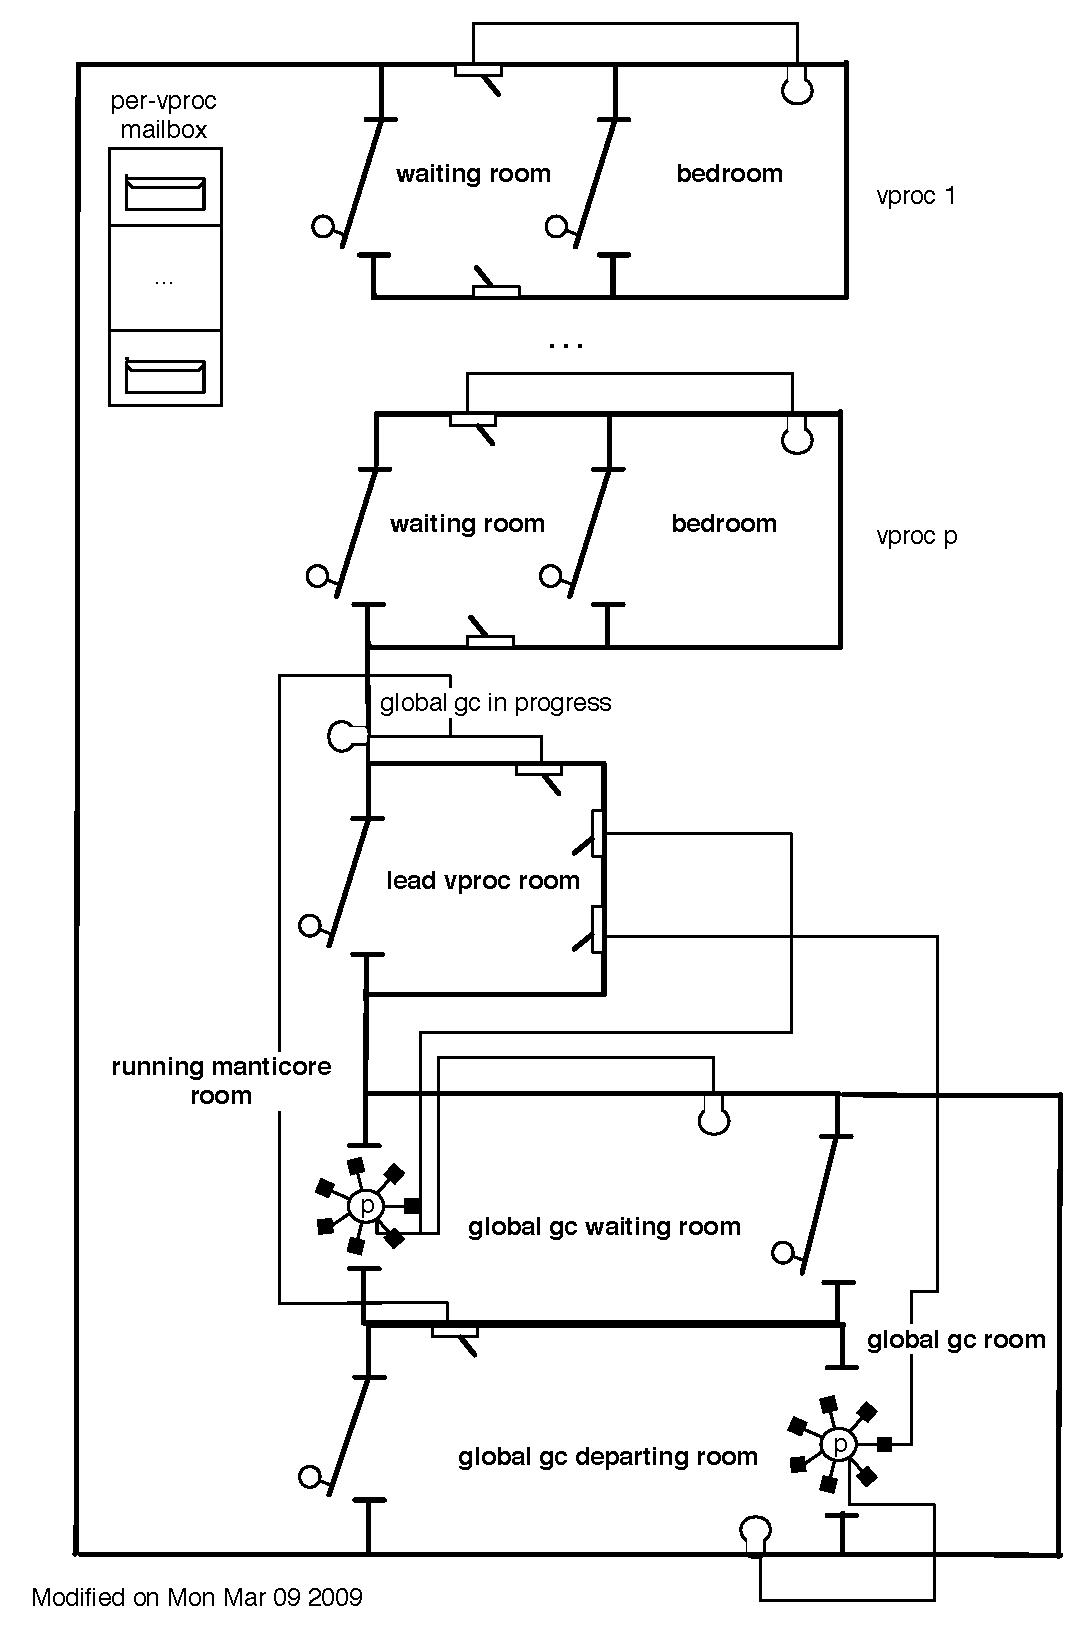
\includegraphics[scale=0.7]{pictures/vproc-protocol}
  \end{center}%
  \caption{Layout of the VProc protocol.}
  \label{fig:vproc-protocol}
\end{figure}%

\section{Messaging}

\paragraph{\texttt{Send(vp, msg)}}
\begin{enumerate}
  \item Walk to \texttt{vp}'s desk and open the mailbox.
    \begin{enumerate}
      \item If there is a \texttt{SLEEPING} message, place \texttt{msg} in the mailbox and go to step 2.
      \item Otherwise, place \texttt{msg} in the mailbox and exit the subroutine.
    \end{enumerate}
  \item Walk into \texttt{vp}'s \textbf{waiting room}.
    \begin{enumerate}
      \item If the waiting-room switch is off, then do the following.
        \begin{enumerate}
          \item Flip the waiting-room switch on.
          \item Walk into \textbf{running manticore room}.
          \item Exit the subroutine.
        \end{enumerate}
      \item If the waiting-room switch is on, then go to step 3.
    \end{enumerate}
  \item Flip the bedroom switch on.
  \item Walk into \textbf{running manticore room}.
\end{enumerate}

\paragraph{\texttt{CheckMailbox()}}

\begin{enumerate}
  \item Walk to the desk and open the mailbox.
  \item Retrieve all messages, leaving the mailbox empty.
  \item Handle each message \texttt{msg}.
\end{enumerate}

\section{Sleeping}

\paragraph{\texttt{Sleep()}}
\begin{enumerate}
  \item Walk to the desk and open the mailbox.
    \begin{itemize}
      \item If empty, place a \texttt{SLEEPING} message in the mailbox.
      \item If nonempty, exit the subroutine.
    \end{itemize}
  \item Walk into the \textbf{waiting room}.
    \begin{itemize}
      \item If the waiting-room switch is on, then go to step 7.
      \item If the waiting-room switch is off, then go to step 3.
    \end{itemize}
  \item Flip the bedroom switch off.
  \item Walk into \textbf{bedroom}.
  \item Wait for the light to turn on.
  \item Walk into \textbf{waiting room}.
  \item Flip the waiting-room switch off.
  \item Walk into \textbf{running manticore room}.
\end{enumerate}

\paragraph{\texttt{Wake(vp)}}

\begin{enumerate}
  \item Construct a blank message \texttt{msg}.
  \item Apply \texttt{Send(vp, msg)} and, once complete, exit the subroutine.
\end{enumerate}

\section{Global GC}

\paragraph{\texttt{GlobalLimit()}}

\begin{enumerate}
  \item Walk into \textbf{leader vproc room}.
    \begin{itemize}
      \item If switch is off, then we assign this vproc as the lead.
        \begin{enumerate}
          \item Reset turnstyles.
          \item Walk into \textbf{running manticore room}.
          \item Go to \texttt{LeaderVProc()}.
        \end{enumerate}
      \item If switch is on, then go to step 2.
    \end{itemize}
  \item Walk into \textbf{global gc waiting room}.
  \item Wait for light to turn on.
  \item Enter \textbf{global gc room}.
  \item When finished with global collection, walk to \textbf{global gc departing room}.
  \item Wait for light to turn on.
  \item Walk into \textbf{running manticore room}.
\end{enumerate}

\paragraph{\texttt{LeaderVProc()}}

\begin{enumerate}
  \item For each vproc \texttt{vp}, apply \texttt{Wake(vp)}.
  \item Walk into \textbf{global gc waiting room}.
  \item Wait for light to turn on.
  \item Walk into \textbf{global gc room}.
  \item When finished with global collection, walk to \textbf{global gc departing room}.
  \item Flip the switch off.
  \item Wait for light to turn on.
  \item Walk into \textbf{running manticore room}.
\end{enumerate}

\end{document}  
